\documentclass[../main]{subfiles}

\graphicspath{{../figures/}}

\begin{document}

\chapter{検証実験}
\label{cp:verification_experiment}
\thispagestyle{empty}
\minitoc
\newpage

\section{はじめに}
\label{sec:vexp_introduction}

\clearpage

\section{身体動作および打球品質の解析}
\label{sec:result_exp2}

\subsection{骨格推定によるフォームの定量化}
\label{subsec:result_exp2_pose}
% 内容：成功時と失敗時のフォームの違い
% （例：インパクト時の体幹の前傾角度、肩のラインの崩れなど）

\subsection{物体検出によるショットマップと着弾分布}
\label{subsec:result_exp2_shotmap}
% 内容：ボールの着弾点の可視化（ヒートマップや散布図）
% IN群は集弾性が高いが、OUT群はばらつきが大きい、などの事実
本実験において計測された前試行におけるボールの着弾位置を卓球台平面上にプロットした結果を図\ref{fig:shotmap}に示す．図中の各プロットの色は\ref{subsec:shotaccuracy}節で定義したターゲットからの誤差距離$D_{err}$に対応している．また黒色の×印は打球がOUTになった時を示している．
図\ref{fig:shotmap}より，被験者の打球の多くはターゲット周辺に集団しており，実験課題であるクロス方向への内訳が遂行されていることが確認できる．
一方で，ターゲットから大きく逸脱した試行（暖色系のプロット）も散見され，打球ごとに精度のばらつきが生じていることがわかる．
特に，着弾点がネットぎわやサイドライン外側に大きく外れるケースでは，打球前の身体ポジションやスイング動作に何かエラーが生じている可能性が示唆される．次節以降では，これらの着弾誤差を教師データとして，その要因を身体動作および筋活動の両面から解析した結果について述べる．

\begin{figure}[h]
    \centering
    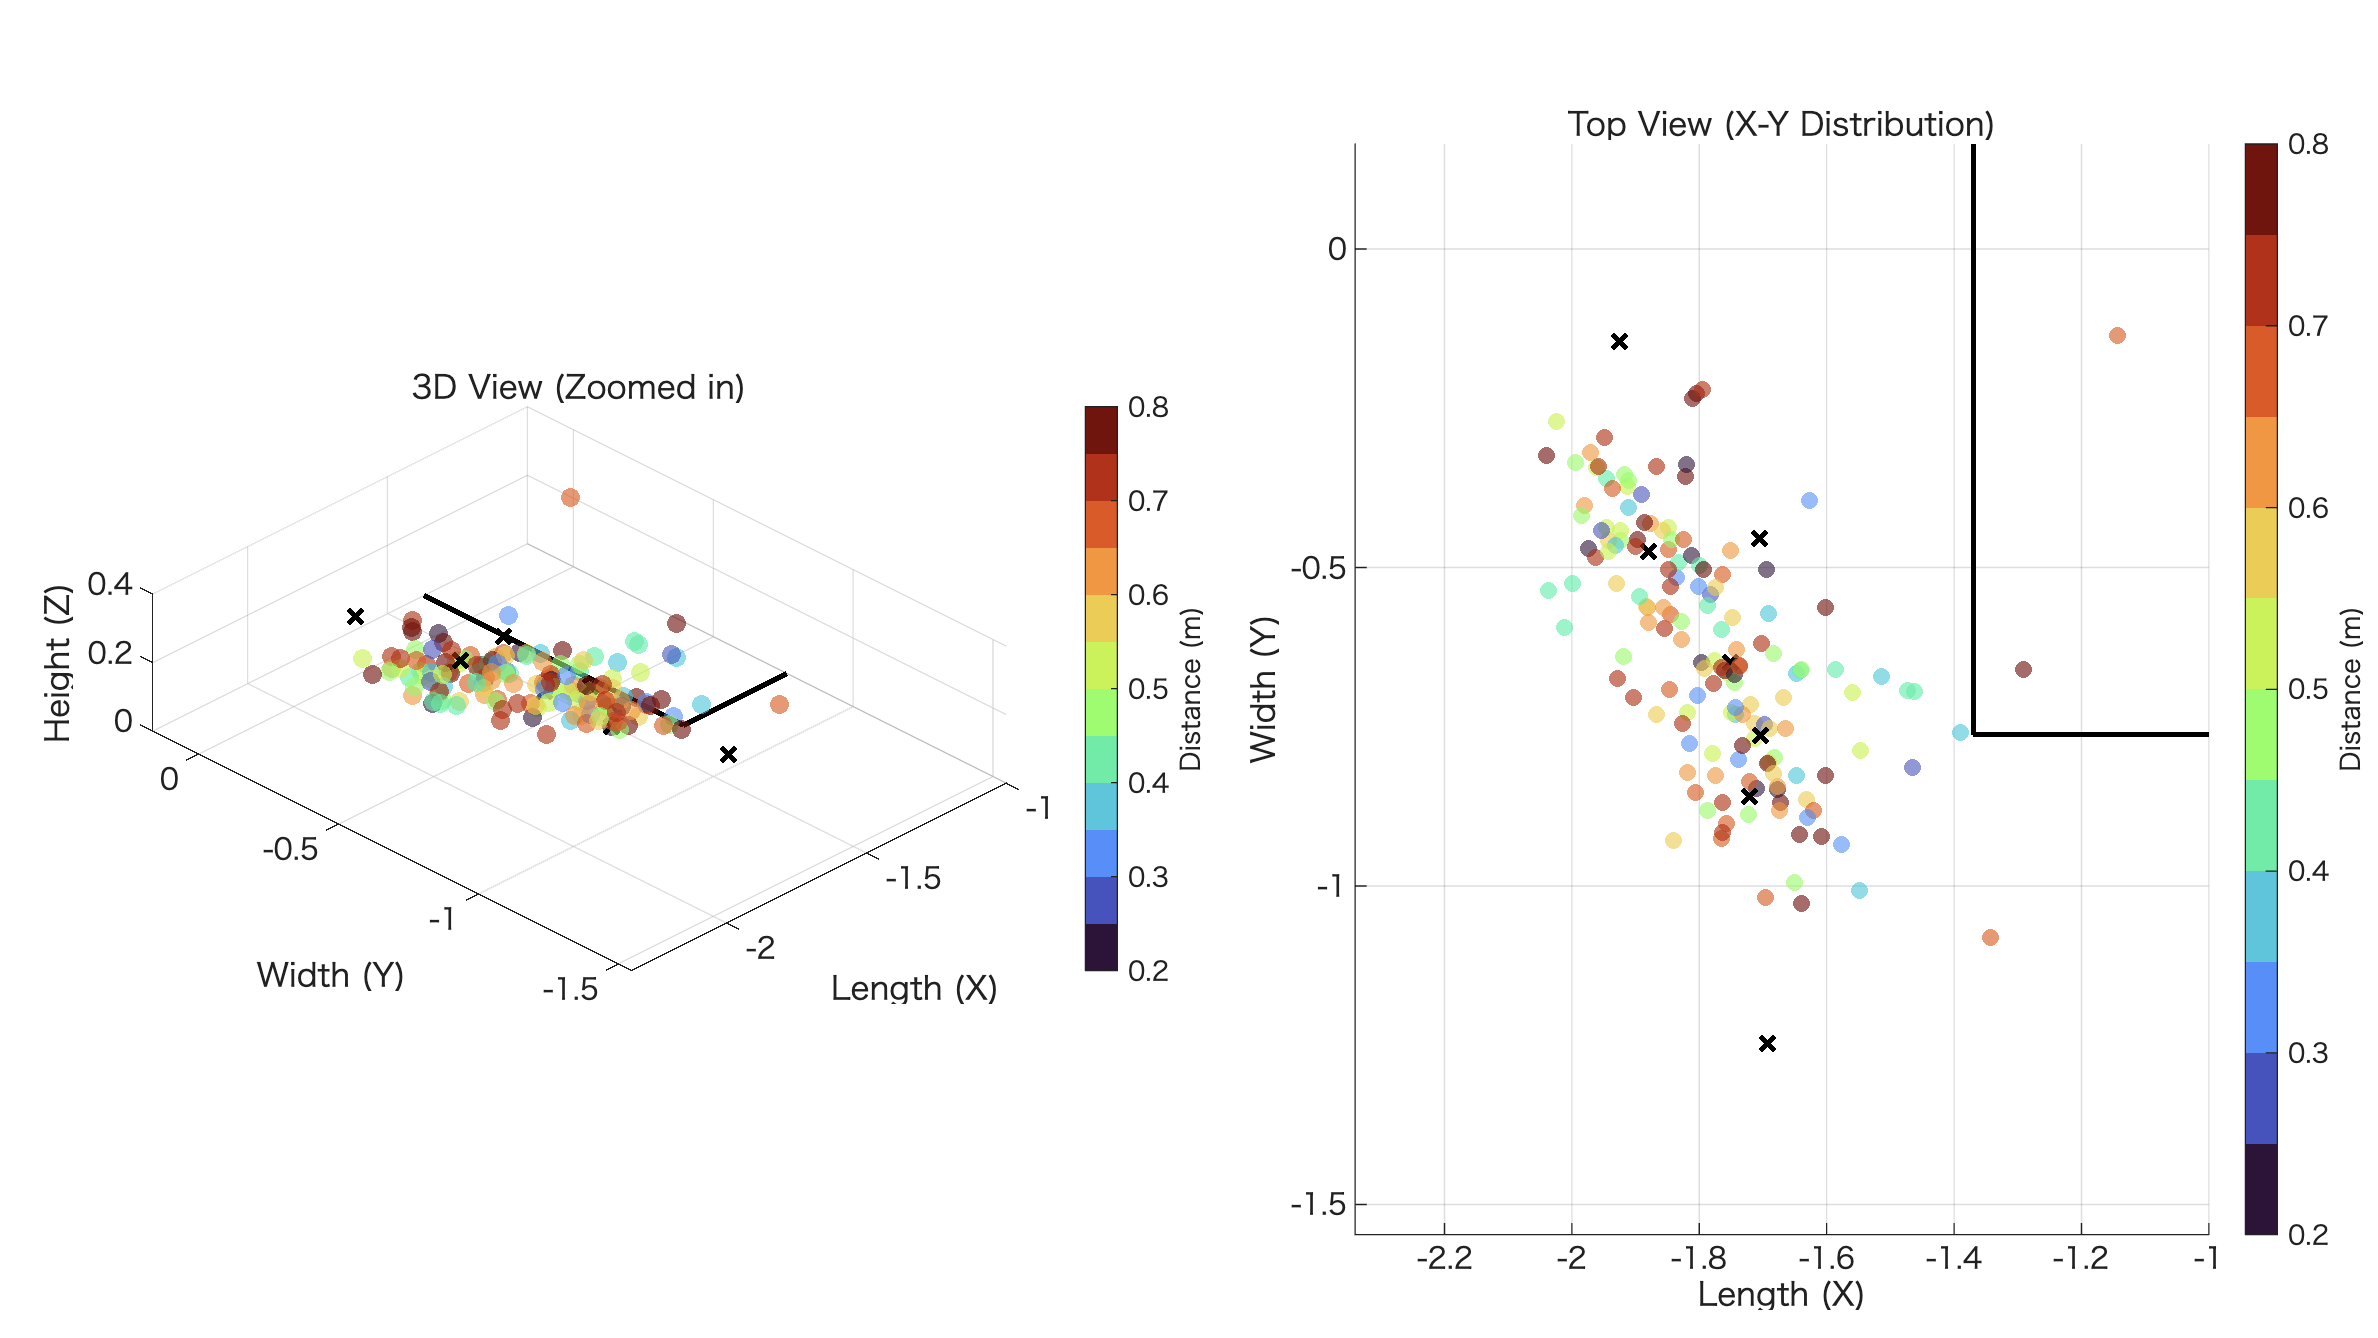
\includegraphics[keepaspectratio, width=1.0\linewidth]{chap3/shotmap.png}
    \caption{打球位置の散布図　色：その打球の着弾点と目標との距離}
    \label{fig:shotmap}
  \end{figure}



\subsection{考察：身体動作の変容とパフォーマンスの関係}
\label{subsec:discussion_exp2}
% 内容：
% ・フォームの崩れが物理的にどうボール軌道に影響したか
% ・着弾点のばらつきから見える、プレーの安定性について

\clearpage

\section{筋活動に基づく打球成否要因の解析}
\label{sec:result_exp1}

\subsection{打球成否の識別精度と有効時間窓}
\label{subsec:result_exp1_accuracy}

\subsection{PFIによる重要筋の特定と時系列パターン}
\label{subsec:result_exp1_muscle}

\subsection{考察：準備段階における筋活動の役割}
\label{subsec:discussion_exp1}

\clearpage

% 3.3節：総合考察（★ここが卒論の要）
    % 2つの実験を「個別最適化」というテーマで統合します
\section{動作解析と筋活動解析の統合的理解}
\label{sec:general_discussion}
% 内容：
% ・実験1（筋活動の遅れ）が、実験2（フォームの崩れ・着弾ミス）にどう繋がったか？
%   （例：「腹斜筋の活動開始が遅れたことで、インパクト時の体幹固定が間に合わず、結果としてフォームが崩れてOUTになった」という因果関係の推察）
% ・本手法を用いることで、選手個人にどのような具体的な指導（個別最適化）が可能になるか？
\clearpage

\section{おわりに}
\label{sec:vexp_conclusion}

\clearpage

\end{document}
